\documentclass[a4paper,10pt]{article}
\usepackage{url}
\usepackage{graphicx}
\usepackage[utf8]{inputenc}
\usepackage[backend=biber,autocite=footnote,notetype=foot+end,style=authortitle-ibid]{biblatex}
\usepackage[colorinlistoftodos]{todonotes}
\usepackage{lipsum}
\bibliography{group4}

\begin{document}

    \title{Cloudy With a Chance of Tweetfall \\ \large{Do Weather Forecasts Influence Sentiment of Posts on Twitter?}}
    \author{
        Johnston, Cian
        \and
        Ravindran, Aishwarya
        \and
        Chavady, George
        \and
        Karode, Sameer
        \and
        Kulkarni, Shravani Deepak
    }

    \maketitle

    \begin{abstract}
     In this paper, we focus on performing sentiment analysis of data retrieved from Twitter with regard to textual categories implicit in local weather forecasts for the year of 2018 in the Republic of Ireland. Season-wise Tweets (Spring, Summer, Autumn and Winter) experienced in Ireland along with sentiments of the weather on a particular day of the season were analyzed. TextBlob was used to measure the sentiment of a Tweet and weather forecast data was categorised as hot, wet and rainy to name a few. No significant results were found between the extracted weather features and the overall sentiment polarity of Tweets in the given time period.
    \\
    \textbf{\textit{Keywords:}} Twitter, sentiment analysis, python, weather forecast, wordnet
    \end{abstract}

    \section{Introduction}

    Sentiment analysis is a critical and essential area because sentiment fundamentally relates to a person’s emotions, impressions, and attitude. Analysing every individual’s sentiment from a text analytics point of view accurately is challenging. It involves trying to comprehend the thoughts and assumptions of an individual with regard to a concept or topic in a particular context, be it positive, negative or neutral \footfullcite{aylien_sentiment}. It is estimated that nearly 2.5 quintillion bytes of data is generated each day \footfullcite{blazon_howmuchdata}, and there is a plethora of information available online relating to a person’s messages, tweets, documents, emails, chats, conversations, and comments. Sentiment analysis allows us to analyse this huge amount of data efficiently.

    
    In this paper, we address the question of whether a correlation exists between textual weather forecasts and the sentiment of posts on Twitter \footfullcite{mining_twitter_data}. Specifically, we focus on performing sentiment analysis of data retrieved from Twitter with regard to textual categories implicit in local weather forecasts for the year of 2018 in the Republic of Ireland. 
    Twitter is an acclaimed stage for social networking, which allows people to express their interests and thoughts online in the form of short posts known as “Tweets”. With over 500 million Tweets per day pertaining to almost any topic, it is an excellent platform for sentiment analysis due to its accessibility and real-time nature of its data. It is not uncommon that weather plays an important role in an individual’s mood and its consequences because of the decisions made. \todo{Add citation}
    
    At a high level, we analyze the Tweets season-wise to understand the general sentiment in the tweets for each of the four seasons that are experienced in Ireland (Spring, Summer, Autumn and Winter). For instance, we compare the Twitter sentiment during the summer months and those in winter. Additionally, at a deeper level, we analyze the tweets for each day and correlate it with the weather on that day. In this case, we find the trends in the sentiments on sunny, cloudy, wet, dry, cold, cloudy and windy days. Furthermore, we also compare these trends on weekdays and weekends. For these analyses, we make use of visualizations to gain more insights into correlations between the weather categories and sentiments.

    The remainder of this paper is laid out as follows:
    \begin{itemize}
        \item{In Section \ref{related_work}, we outline some related work already peformed in this field.}
        \item{In Section \ref{methodology}, we describe the processes of obtaining and analyzing the data.}
        \item{In Section \ref{results}, we give an overview of the results of our analyses.}
        \item{Finally, Section \ref{conclusion} provides a summary and evaluation of our findings.}
    \end{itemize}


    \section{Related Work}
    \label{related_work}

    As accessibility to real-time information increases, performing analysis on this kind of data becomes more viable. There has been a lot of notable research done on sentiment analysis of Twitter data in general. Park et al. find a correlation between weather and people’s mood and sentiments from Twitter data by measuring temperature, humidity and atmospheric pressure \footfullcite{park2013mood}. These weather variables seem to have a satisfactory impact on one’s mood. Bagheri et al. \footfullcite{bagheri2017sentiment} focuses on implementing sentiment analysis on Twitter data using the Twitter APIs and a wealth of available libraries. Tweets are well-known for including abbreviations and colloquialisms, making it challenging to extract polarities from these texts. Deep Learning image classifier could be utilised to predict the sentiment of an image as positive (e.g. a colourful balloons) or negative (e.g. a missile). According to Dang, N.C et al. latest studies have employed deep learning to solve sentiment analysis problems, such as sentiment polarity \cite{dang2020sentiment}.
    
    Sentiment analysis has been applied to various areas including, but not limited to, elections, politics, movie ratings, and fashion. In 2015, Chen et al. performed notable research in the area of predicting future crime rates in Chicago, IL, using GPS tagged Twitter data \footfullcite{chen2015crime}. They aimed to predict the time and location during which a specific type of crime is expected to occur by applying lexicon-based sentiment analysis on categorized weather data combined with kernel density estimation of historical crime incidents, and were able to test their model's ability to predict future crime on each area of the city. Hannak et al. \footfullcite{hannak2012tweetin} concentrated on using a Twitter-specific sentiment extraction methodology and explored a corpus of over 1.5 billion Tweets. With the help of machine learning techniques on this corpus, correlating with the weather at a particular time and location of the Tweets, they concluded that aggregate sentiment follows different climate and seasonal patterns.

    \section{Methodology}
    \label{methodology}

    Our hypothesis states that there exists a significant correlation between the overall sentiment of Tweets at a given time, and the features of a given textual weather forecast for the same specified time on which that Tweet was posted. Therefore making our null hypothesis is that no significant correlation exists. In order to address the hypothesis, two sources of data were procured: a collection of posts from Twitter, and a collection of textual weather forecast data. Both of these corpora were assembled and filtered such that they both relate to the same geographical area, and to the same duration of time. The geographical area in question was restricted to the Republic of Ireland, and the time-span in question was limited to the year of 2018. 

    \subsection{Twitter Data}

    \subsubsection{What to measure}

    To measure the sentiment of a Tweet, we elected to use the \texttt{TextBlob} \footfullcite{textblob_doc} library, which internally utilises a Naive Bayes classifier pre-trained on a corpus of movie reviews. Applying this classifier to a text yields a tuple of two real-valued integers in the range [-1.0, 1.0], denoting both the \textit{polarity} and the \textit{subjectivity} of the text.

    Textual weather forecasts cannot be correlated directly with Tweet sentiment. In order to perform some meaningful analysis, we defined a number of weather-related categories of interest and determined how strongly a given weather forecast applied one of those categories. The categories chosen were cold, hot, wet, dry, cloudy, and windy. For example, the forecast ``Some sunny spells giving way to scattered showers later on'' relates both to \texttt{SUNNY} and \texttt{WET} categories.

    \subsubsection{Data Collection}

    Twitter provides an API for developers to both read data and interact with users. This has a number of limitations, including rate limits \footfullcite{twitter_api_docs_rate_limit}, and a requirement to request an API key. In order to access a useful volume of data, this would require a large number of HTTP requests to Twitter. Thankfully, the Internet Archive provides a large dataset of posts on Twitter for the year of 2018 in TAR format \footfullcite{archiveorg_twitter}. While these datasets are essentially a subset of the \textit{global} content of Twitter, and technically much larger than required, they are hosted using BitTorrent and are thus much more straightforward to download. For the purposes of this paper, we elected to use a subset of the Twitter archive data from the year 2018.

    \subsubsection{Data Processing}

    The large archives detailed above needed to be preprocessed before any meaningful analysis can be performed. To this end, a small program was written to consume the entire TAR archive and filter out Tweets matching certain criteria, serializing a subset of the data to CSV format. This was done to avoid extracting the entire archive to disk, which is a time-consuming operation. The following criteria were used for extracting Tweets of interest:
    \begin{itemize}
        \item{
            Having geo-location information within Ireland, or
        }
        \item{
            Posted by a user with user-specified location containing the string \textit{Ireland}.
        }
    \end{itemize}

    Note that not all Tweets posted by users in Ireland will necessarily have geo-location information attached, and not all Tweets posted by users claiming to be located within Ireland are necessarily so.

    \subsubsection{Data Cleaning}

    The tweets are 140 characters long. Considering this constraint, initial analysis from the chunk of tweets revealed that, users tend to use more contractions and emojis to express their thoughts rather than using appropriate grammar. The sentiment score given by the existing implementations like TextBlob is affected by the use of such text. We implemented a python code to do the preprocessing of the data obtained, which is obtained using Twitter API.

    The filtering process removes the URLs, usernames, and hashtags. In some situations, it is known that hashtags can provide instant insight as to what the users are feeling. However, most hashtags that we encountered contain meaningless text or sentences for tags instead of keywords.
    % The process flow is illustrated in Figure \ref{fig:twitter_process_flow}.

    % \begin{figure}
    %     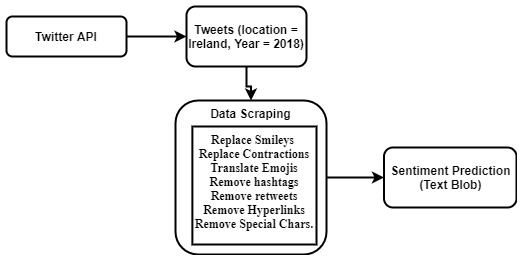
\includegraphics[width=0.8\textwidth]{twitter_process_flow.jpg}
    %     \caption{Twitter data processing flow.}
    %     \label{fig:twitter_process_flow}
    % \end{figure}

    \begin{itemize}
        \item{
            We removed hashtags, retweets, @mentions, hyperlinks and special characters using regular expressions.
                    }
        \item{
            Next, we replaced all the contractions in the tweets to its original forms. We used a dictionary of all the contractions with its original form and replaced them in the text.
            
        }
        \item{
            Lastly, we translated all the emojis/smileys to texts. For the smileys using special characters, we used the same approach as in the previous step (a dictionary containing the smileys and their corresponding meaning). We utilized the emoji library available in python for this conversion.
        }\end{itemize}



    \subsection{Weather Data}

    \subsubsection{What to measure}

    For the purposes of our hypothesis, given a textual weather forecast and a finite set of potential features of weather forecasts, we map each textual forecast to a subset of those potential features. As stated previously, the features chosen were cold, hot, wet, dry, cloudy, and windy. To perform the mapping, we count the occurrences of concepts relating to each of those features in the text using \texttt{textblob} and WordNet \footfullcite{fellbaum2012wordnet}.

    \subsubsection{Data Collection}

    Some historical weather data was collected from MET \'{E}ireann, the Irish National Meteorological Service. \footfullcite{metie}. Unfortunately, historical textual weather forecast data is not available from MET \'{E}ireann; to work around this, we used the Internet Archive's Wayback Machine \footfullcite{wayback_machine} to access previously published versions of the MET \'{E}ireann homepage which contains daily textual forecast data.

    To access previously versions of the website more conveniently, the tool \texttt{wayback-machine-scraper} was utilised \footfullcite{github_sangaline_wayback-machine-scraper}. This is a command-line utility that interfaces with \textit{Wayback Machine} and allows a user to download a number of snapshots of a website for a specified date range. For the purposes of this paper, we fetched all the saved snapshots of the MET \'{E}ireann homepage for the year of 2018. Note that this is a sparse dataset, and snapshots of this data is not available for every day.

    As an alternative source of textual forecast data, we turned to a more unorthodox source -- Boards.ie is a discussion board with a wide range of fora which, naturally, includes the topic of weather. One particular thread of interest on this sub-forum has almost daily forecasts provided by an amateur meteorologist with the moniker 'M.T. Cranium' \footfullcite{boards_ie_mt_cranium_forecasts}. The relevant print versions of the thread spanning the year of 2018 were saved, and the relevant daily forecasts were extracted using a Python script. 
    % The process is illustrated below in Figure \ref{fig:weather_process_flow}.

    % \begin{figure}
    %     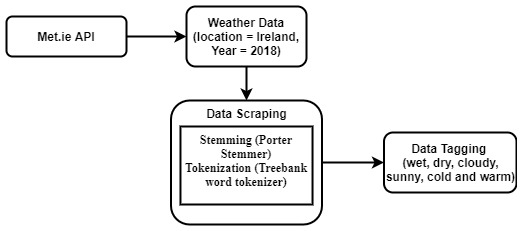
\includegraphics[width=0.8\textwidth]{weather_process_flow.jpeg}
    %     \caption{Weather data processing flow.}
    %     \label{fig:weather_process_flow}
    % \end{figure}


    \subsubsection{Data Processing}

    The textual forecast data on its own needs to be processed before any meaningful correlations can take place. To this end, we utilised the \texttt{TextBlob} library to perform the following:
    \begin{itemize}
        \item{
            Stemming and tokenization of the raw text. TextBlob leverages NLTK's pre-implemented stemmers and tokenizers for the English language, and also uses NLTK's WordNet integration to provide the senses of each individual word in a sentence.
        }
        \item{
            Annotation of the tokenized forecast data with some predefined features. We first define a number of top-level concepts: \textit{cold}, \textit{hot}, \textit{wet}, \textit{dry}, \textit{cloudy}, and \textit{windy}. For each of these concepts, we define a set of related \textit{senses} to this concept. We take the sense itself, and all of its children, or \textit{hyponyms}. Then, we compute the intersection of both the set of senses for a given word in the sentence as provided by \texttt{TextBlob}, and the set of senses for the given concept. We then count the number of such overlaps as the measure of the relatedness of the given text to the given concept. \\
            For example, given the sentence ``Very cold and frosty tonight'', we can extract the senses \texttt{cold.a.01} and \texttt{frosty.s.02}, and count two instances of sense overlaps with the concept of \textit{cold}. These features were then extracted for all of the collected forecast data and serialized to CSV format.
        }
    \end{itemize}

	\subsection{Sentiment Analysis}
	
	After preprocessing of the tweet corpus, the same is processed for carrying out the sentiment analysis. Initially, the text corpus is processed using TextBlob, which is a python library built over Natural Language Toolkit(NLTK). TextBlob provides a sufficient set of tools for performing tasks like Sentiment Extraction, Spelling Correction and Detection of Language. There are two types of sentiment analyzers, by default, the TextBlob uses PatternAnalyzer and second is NaiveBayesAnalyzer. The next steps are to evaluate the sentiment score given by the default and overridden implementation of Analyzer. 


    \section{Results}
    \label{results}

    The weather forecast data collected is annotated with the features \textit{cold}, \textit{hot}, \textit{wet}, \textit{dry}, \textit{cloudy}, and \textit{windy}. The Tweets, annotated with their respective sentiment polarity and subjectivity scores, are joined together with the annotated weather forecast data by their respective posting or publication dates.
    
    Firstly, a high-level overiew of the data was prepared by classifying the Tweet polarity into \textit{positive}, \textit{neutral}, or \textit{negative} categories. The weather forecasts corresponding to the Tweets were additionally categorised into the most frequent category of words occurring in the forecast. This is shown in Figure \ref{fig:analysis_sentiment_weather}. It is evident that the overall proportions of Tweet sentiments remain the same, with the vast majority of Tweets being neutral in sentiment, and only a small proportion having positive sentiment. It was also found that Tweets showed a slightly more positive sentiment of 14.4 percent in hot weather conditions when compared 13.9 percent in cold weather conditions. Also, it was noted that 41.1 percent of the total Tweets had negative sentiment in them during cold weather conditions when compared to 39.2 percent negative sentiment in tweets during wet weather conditions. 

    \begin{figure}
        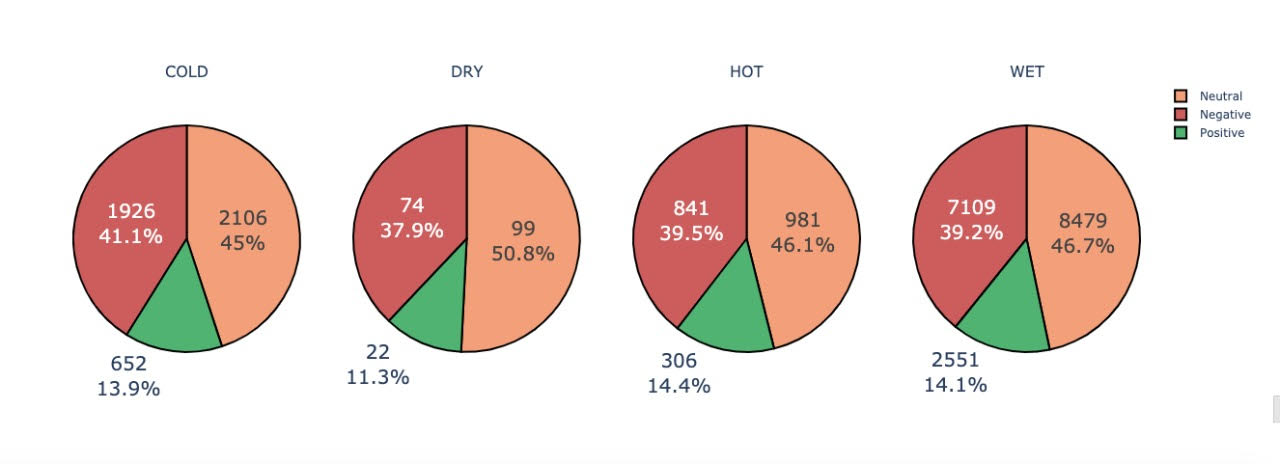
\includegraphics[width=0.8\textwidth]{analysis_sentiment_weather.jpg}
        \caption{Sentiment Analysis of Tweets based on Weather Forecasts}
        \label{fig:analysis_sentiment_weather}
    \end{figure}
    
    The Tweets during weekdays and weekends were also analysed to check for differences. No significant differences were found between sentiment of Tweets posted during weekdays and sentiment of tweets posted during weekends. The results of the analysis is presented in Figure \ref{fig:sentiment_weekdays_weekends}. The box-plot showcasing the sentiment in Tweets takes values that are in the range $[-1, 1]$, where -1 is a completely negative sentiment, +1 is a completely positive sentiment and 0 means neutral sentiment.

    \begin{figure}
        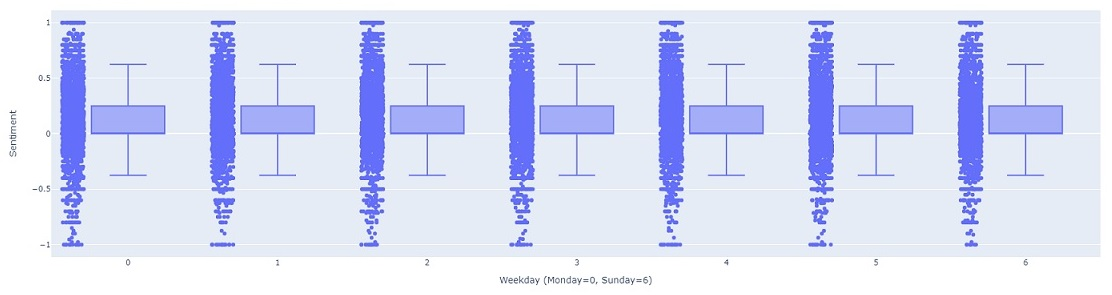
\includegraphics[width=1\textwidth]{sentiment_analysis_weekdays_weekends.jpg}
        \caption{Sentiment Analysis of Tweets on Weekdays and Weekends}
        \label{fig:sentiment_weekdays_weekends}
    \end{figure} 
    
    Finally, Spearman-Rho correlations were calculated for each of the weather features. The numerical results are summarised in Figure \ref{fig:stats1} and Figure \ref{fig:stats2}.

    \begin{figure}
        \begin{tabular}{ l | r  r  r  r  r  r  r  r }
            & \textbf{$\mu$} & \textbf{50\%} & \textbf{25\%} & \textbf{75\%} & \textbf{$\sigma$} & \textbf{Min.} & \textbf{Max.} \\
            \hline
            & \multicolumn{7}{}{} \\
            & \multicolumn{7}{|l}{\textbf{Tweet Sentiment}} \\
            \hline
            \textit{polarity} & 0.115 & 0.000 & 0.000 & 0.250 & 0.303 & -1.000 & 1.000 \\
            \textit{subjectivity} & 0.324 & 0.267 & 0.000 & 0.600 & 0.337 & 0.000 & 1.000 \\
            \hline
            & \multicolumn{7}{}{} \\
            & \multicolumn{7}{l}{\textbf{Counts of Weather Senses}} \\
            \hline
            \textit{cold} & 0.854 & 0.000 & 0.000 & 1.000 & 1.576 & 0.000 & 11.000\\
            \textit{hot} & 0.169 & 0.000 & 0.000 & 0.000 & 0.442 & 0.000 & 3.000\\
            \textit{wet} & 2.316 & 2.000 & 1.000 & 3.000 & 2.127 & 0.000 & 11.000\\
            \textit{dry} & 0.185 & 0.000 & 0.000 & 1.000 & 0.433 & 0.000 & 3.000\\
            \textit{cloudy} & 0.910 & 1.000 & 0.000 & 0.000 & 0.951 & 0.000 & 5.000\\
            \textit{windy} & 1.716 & 1.000 & 0.000 & 2.000 & 1.839 & 0.000 & 14.000\\
        \end{tabular}
        \caption{Descriptive statistics of results.}
        \label{fig:stats1}
    \end{figure}

    \begin{figure}
        \begin{tabular}{l | r r r }
        \hline
        \textbf{Feature} & \textbf{$N > 0$} & \textbf{Spearman-$\rho$} & \textbf{p-value} \\
        \hline
        \textit{cold} & 9,697 & 0.010 & 0.109 \\
        \textit{hot} & 3,606 & -0.001 & 0.869 \\
        \textit{wet} & 21,877 & -0.005 & 0.406 \\
        \textit{dry} & 4,290 & 0.003 & 0.686 \\
        \textit{cloudy} & 15,976 & 0.012 & 0.043 \\
        \textit{windy} & 18,456 & -0.008 & 0.221 \\
        \end{tabular}
        \caption{Spearman-Rho Correlation of Tweet polarity and weather senses.}
        \label{fig:stats2}
    \end{figure}
    
    It was noted that a strong positive correlation of $0.35$ existed between the numbers of occurrences of the \textit{cold} features and \textit{wet} features in the forecast data ($p<0.01$). This is hardly a surprising result, but serves as a sanity check of our methodology thus far.

    Additionally, a minor positive correlation was noted between sentiment polarity and occurrences of \textit{cloudy} senses, but the significance of this relationship does not seem high enough to warrant further investigation. Other relationships are not statistically significant.

    \section{Conclusions and Future Work}
    \label{conclusion}
     Large amounts of data is readily available on Twitter which can be used to analyze sentiment of users' tweets. Also, historical and real time weather data is made available by the meteorological department. We could use weather data and analyze it together with the tweets to predict sentiment for a particular weather forecast using Machine Learning algorithms. Studies have shown that weather conditions such as temperature, precipitation, cloud cover, wind speed and humidity each significantly relate to the expression of sentiment in social media such as Twitter and Facebook. Analysis of sentiment correlated with weather data gives us some important background information of the users of the system, which could be very useful in decision making.

     Possible future prospects might involve collecting Twitter data posted during different seasons of the year and correlating them with actual weather data rather than weather forecasts. More specifically, when the weather data collected is disparate. This data would help us in gauging the effects of weather on Twitter posts.  For example, an increase in temperature from lower values to values between 15C and 20C are associated with significant increases in positive expressions. On the contrary, the number of expressions of positive sentiment decline when the temperature exceeds a value of 30C. There is beneficial scope for performing similar analysis on countries where the weather is more stable so that data can be checked for correlation more efficiently.

    \printbibliography

\end{document}
